\graphicspath{{Appendices/apx1_signal_est}}
\subsection{Power Spectral Density of Individual Truck Signals}

\begin{multicols}{2}
       \begin{figure}[H]
        \centering
        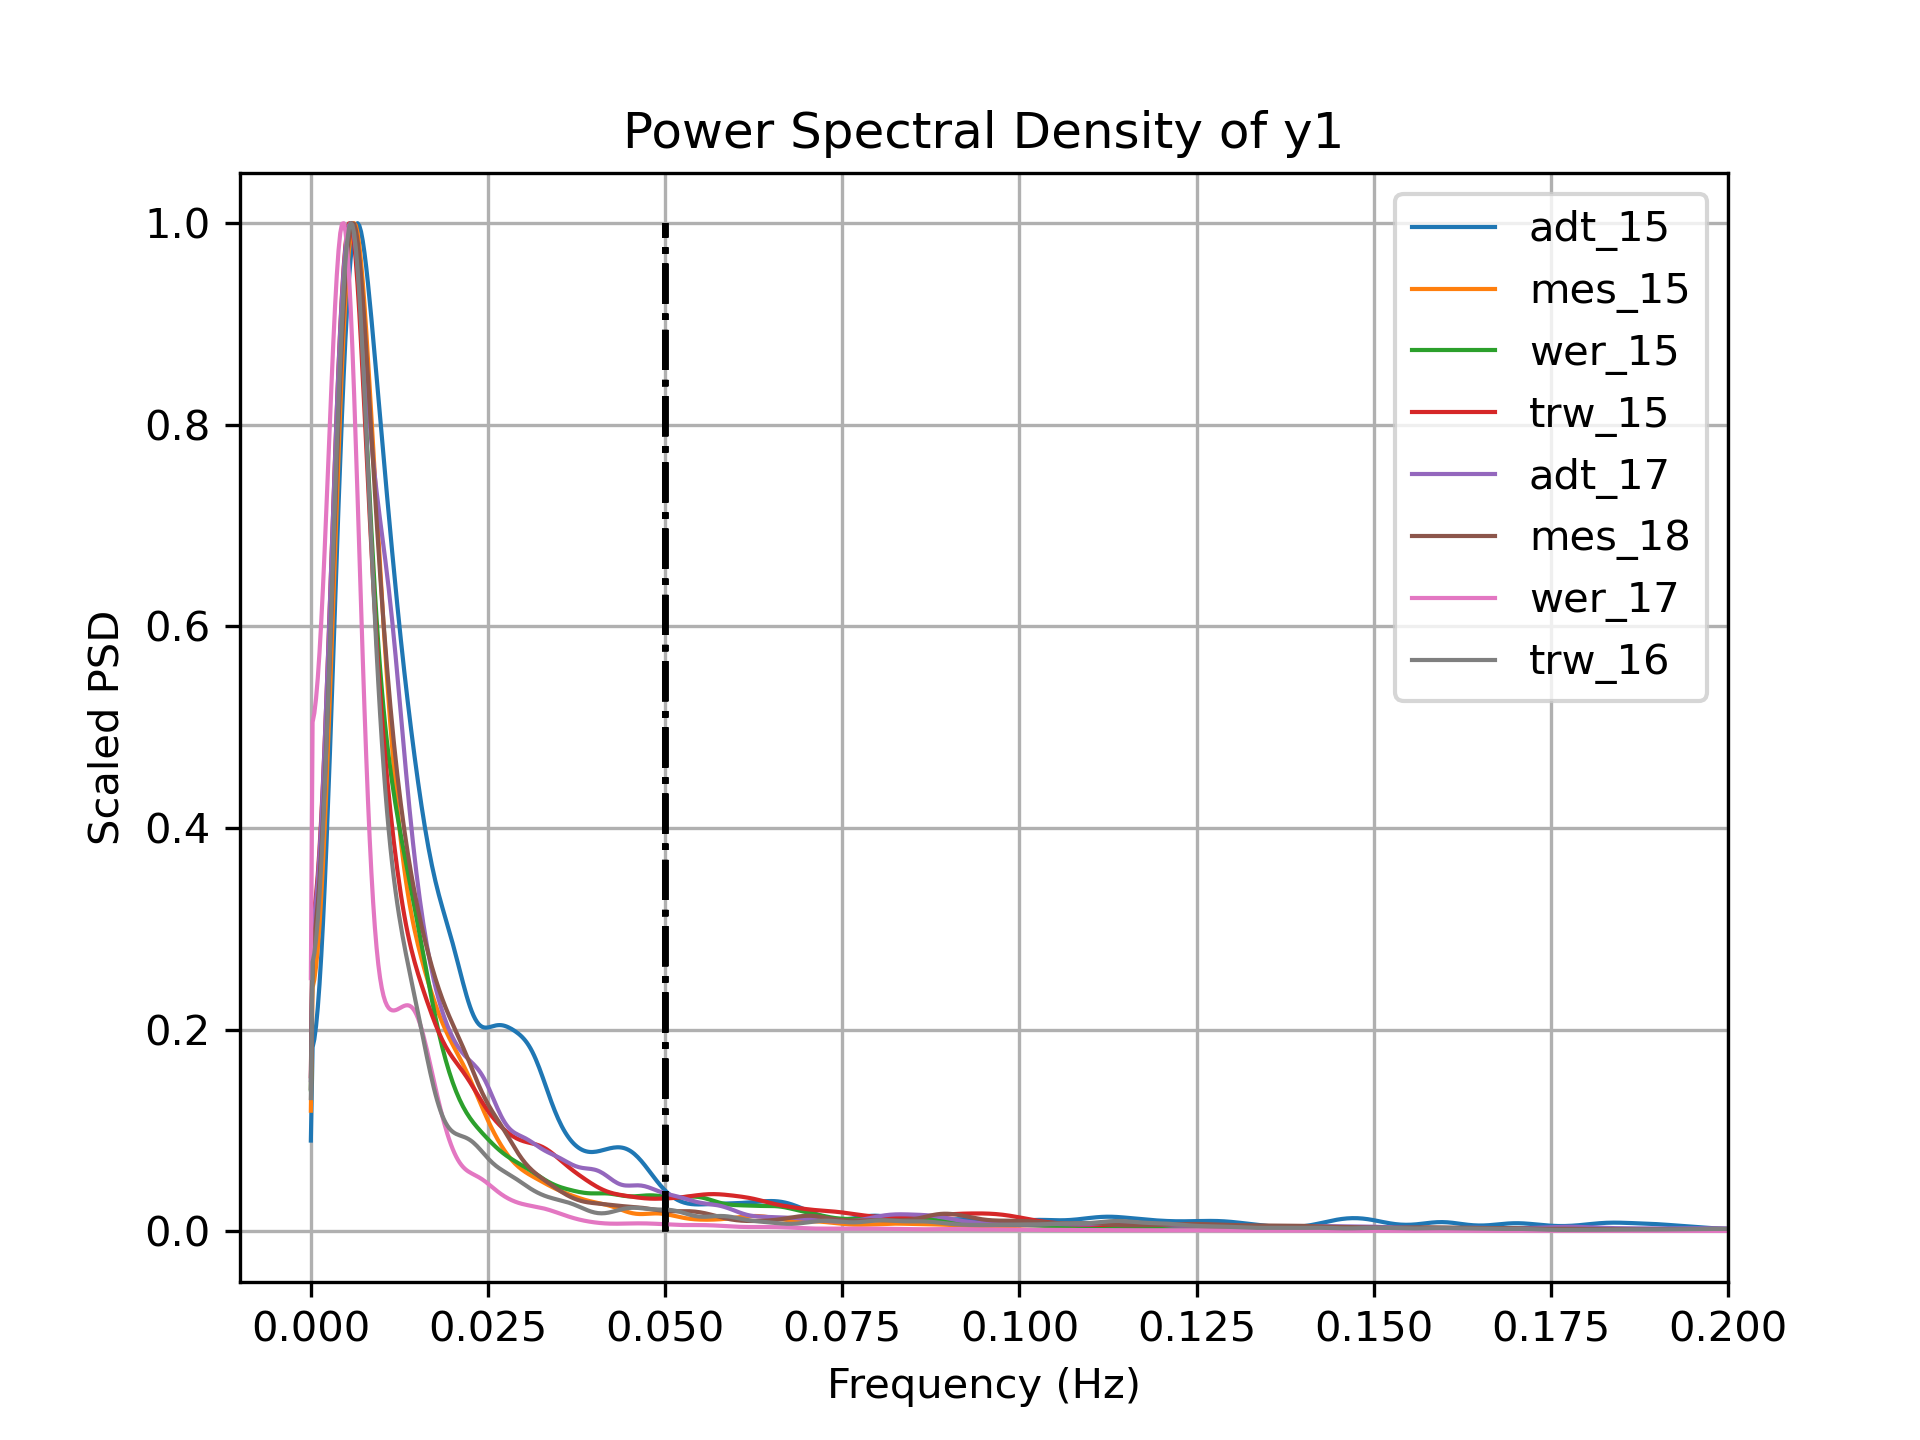
\includegraphics[width=0.48\textwidth]{./figs/bfr_smth/truck_psd/y1.png}
        \caption{PSD of $[NO_x]^{out}$}
       \end{figure}

       \begin{figure}[H]
        \centering
        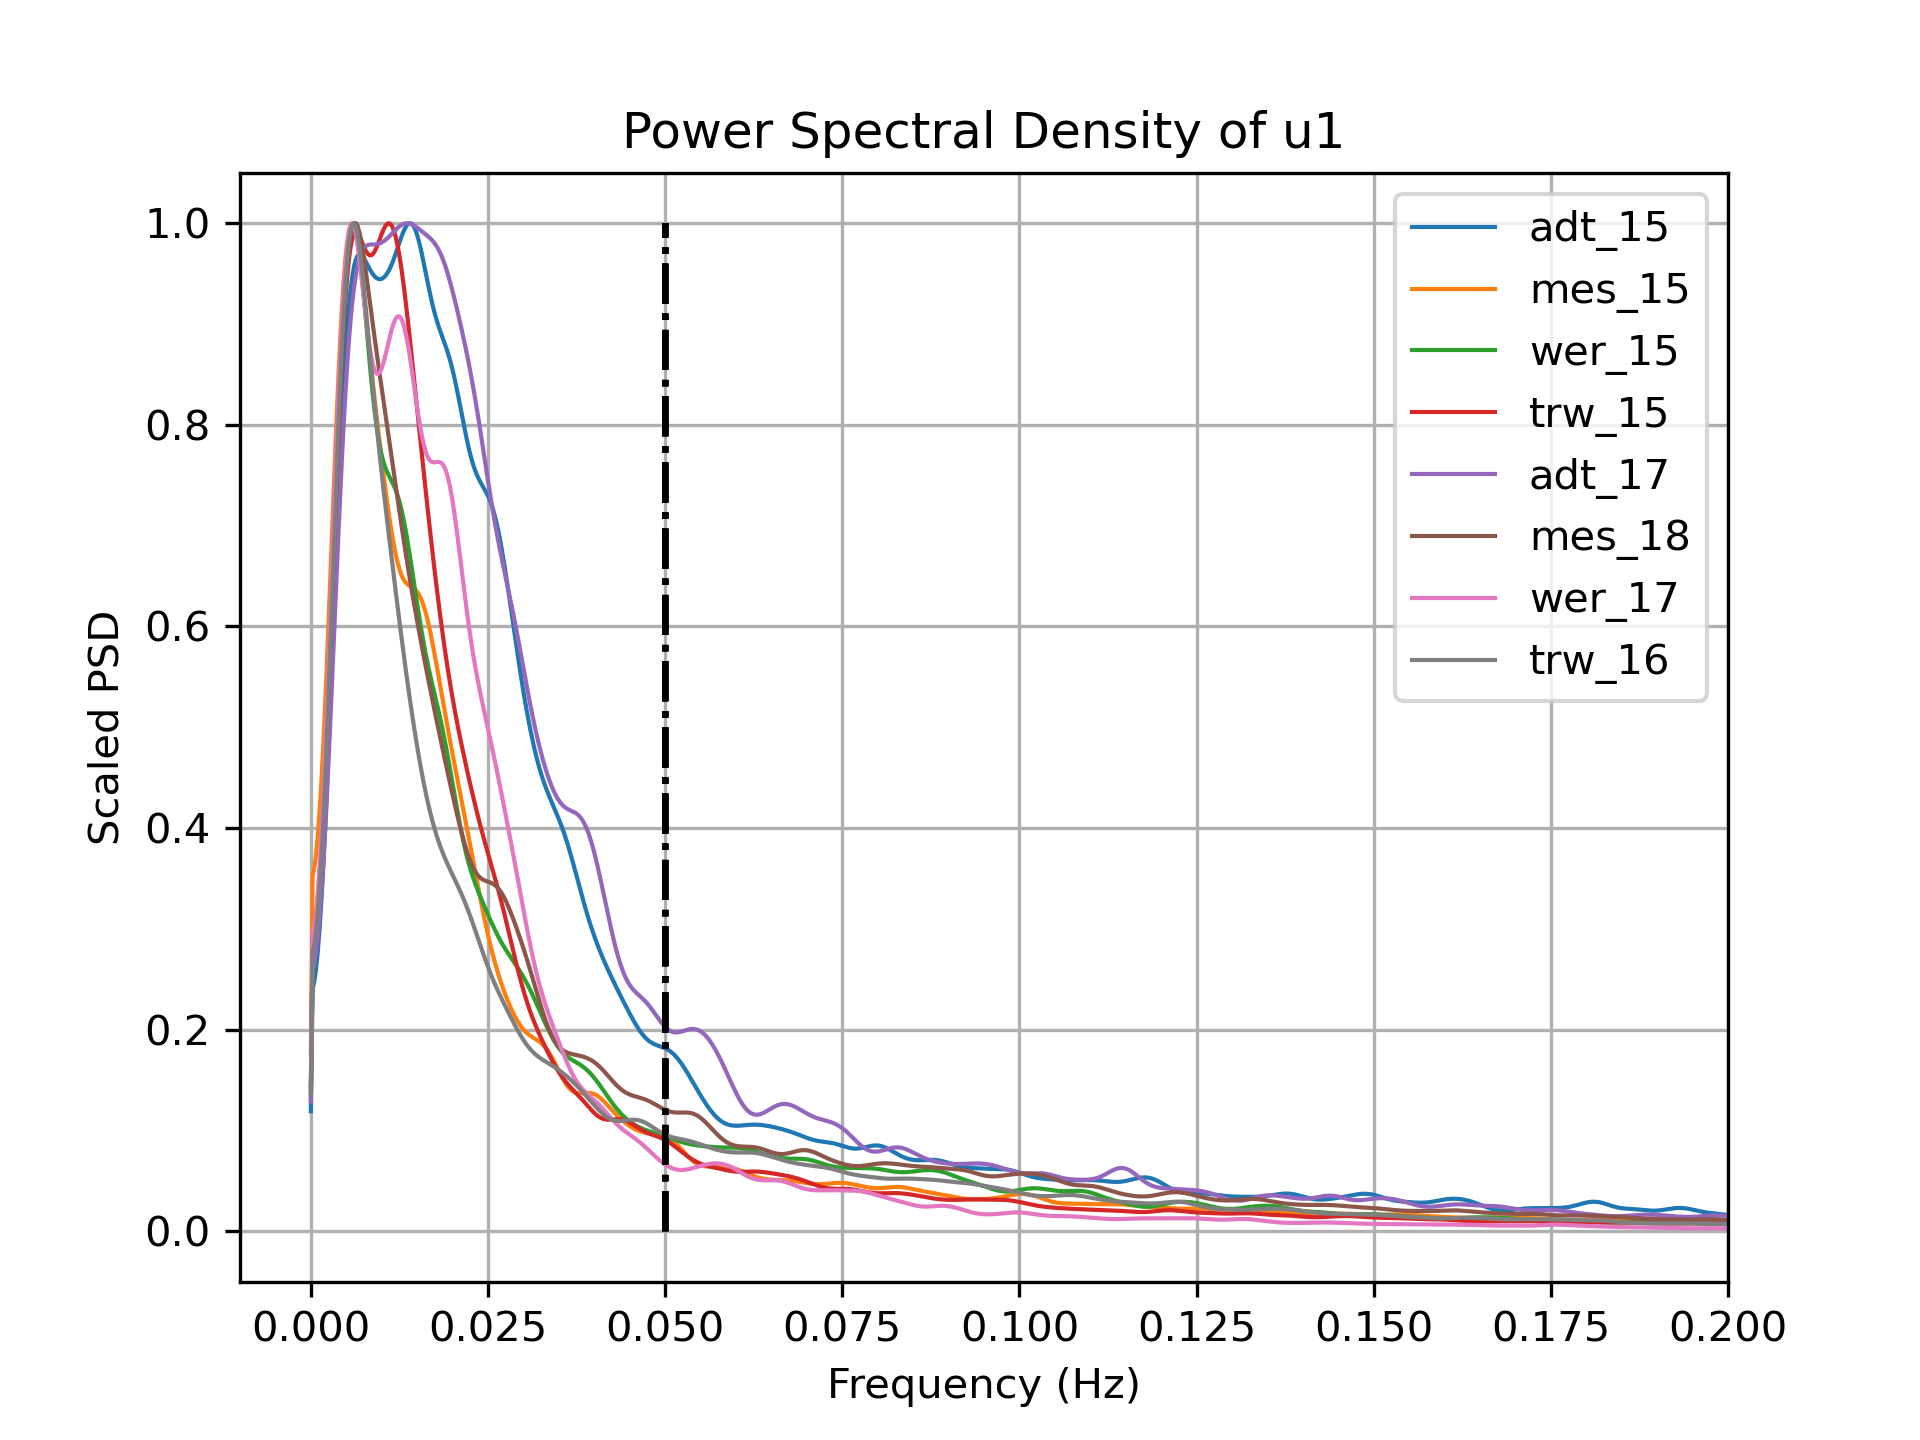
\includegraphics[width=0.48\textwidth]{./figs/bfr_smth/truck_psd/u1.png}
        \caption{PSD of $[NO_x]^{in}$}
       \end{figure}
\end{multicols}

\begin{multicols}{2}
       \begin{figure}[H]
        \centering
        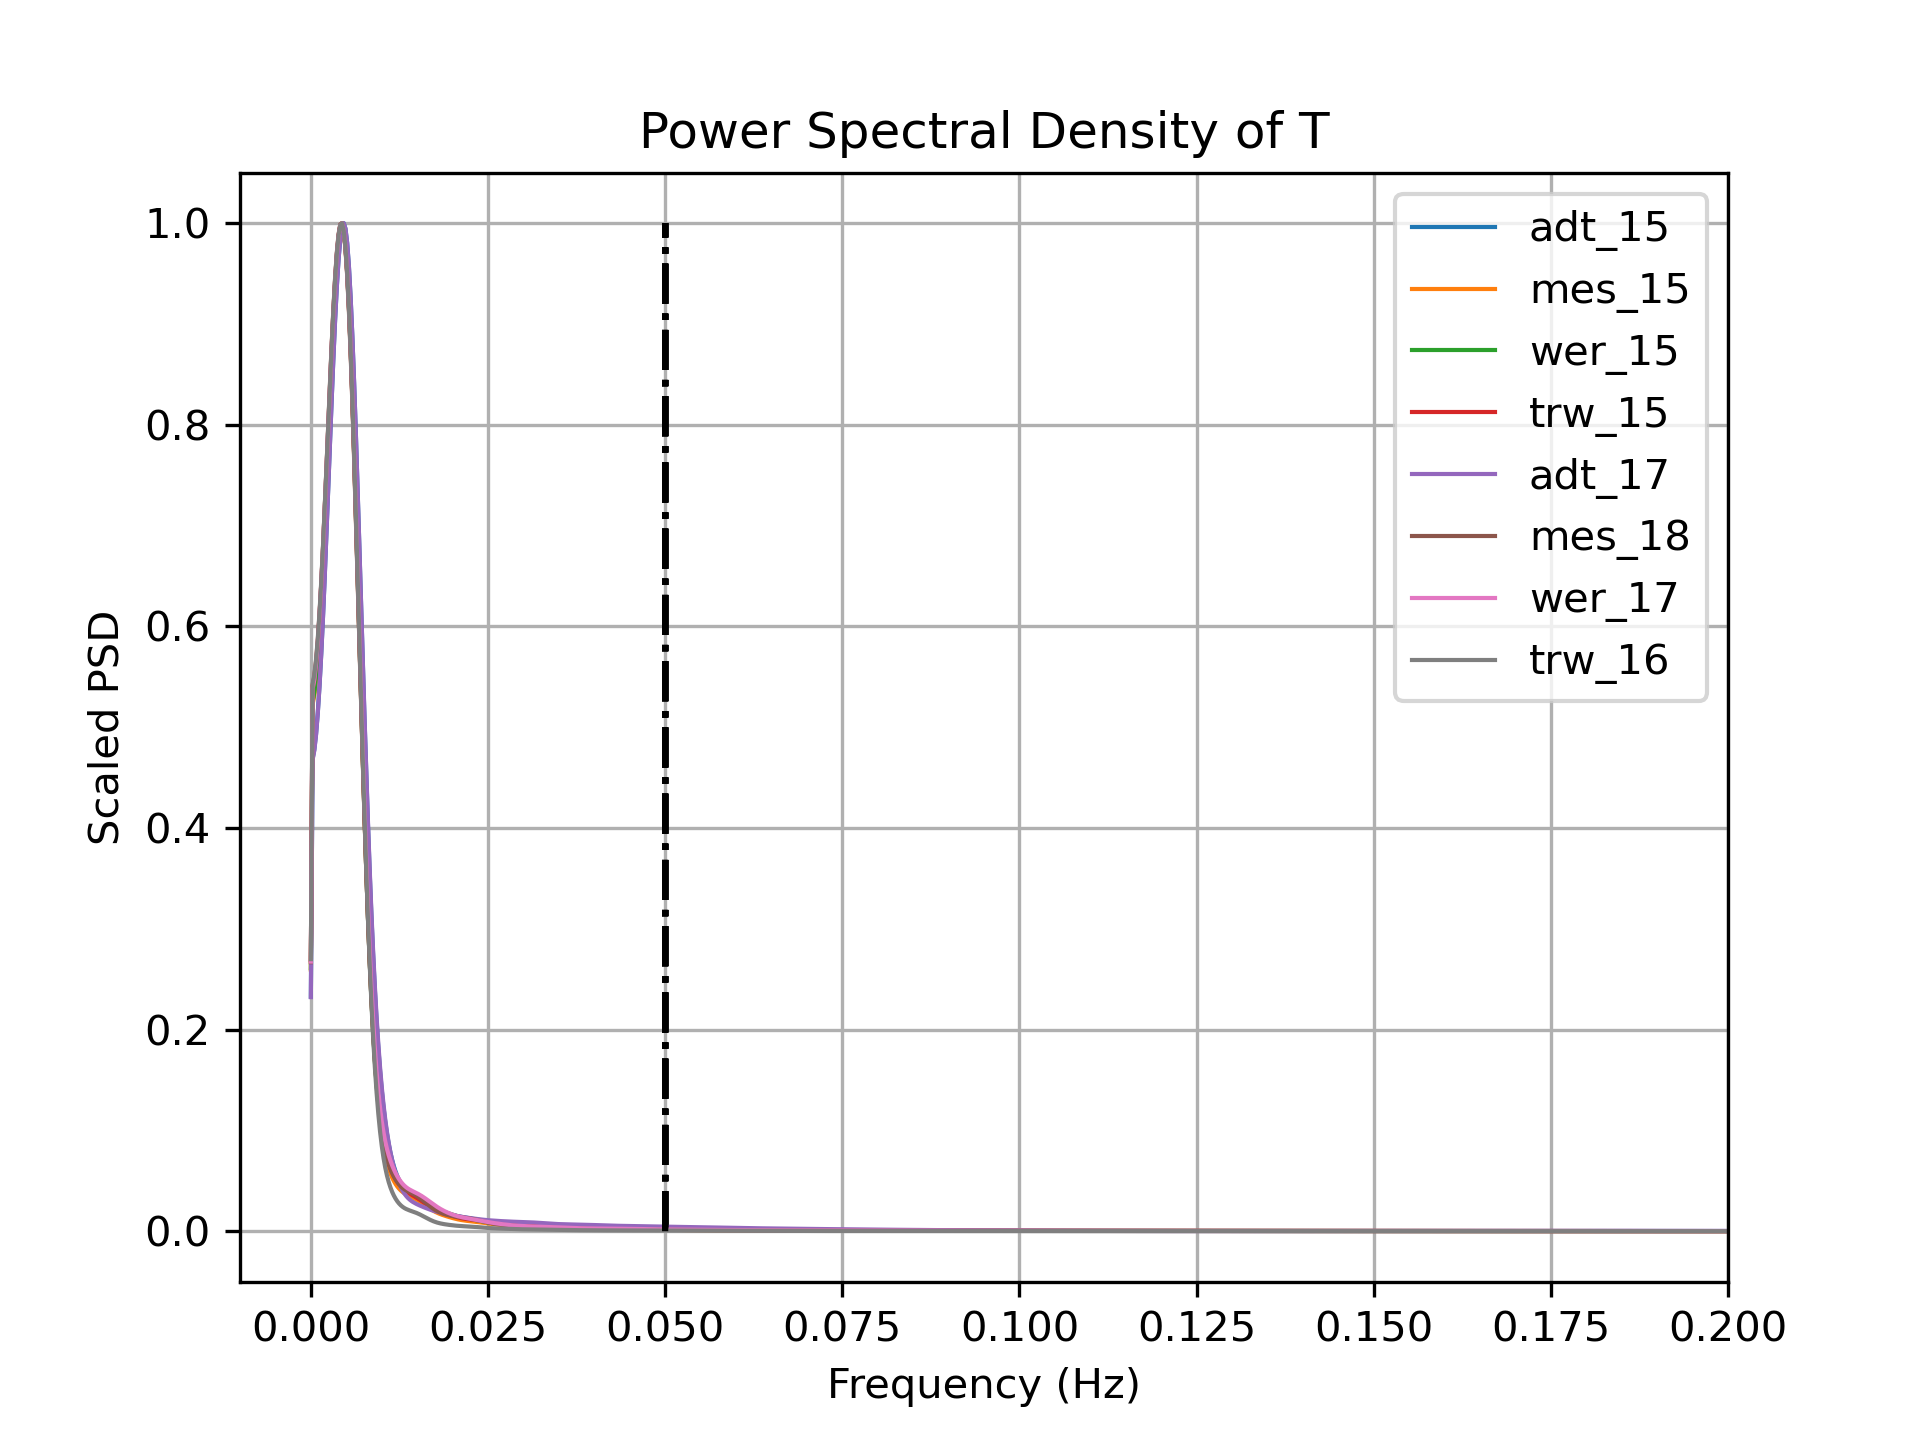
\includegraphics[width=0.48\textwidth]{./figs/bfr_smth/truck_psd/T.png}
        \caption{PSD of temperature}
       \end{figure}

       \begin{figure}[H]
        \centering
        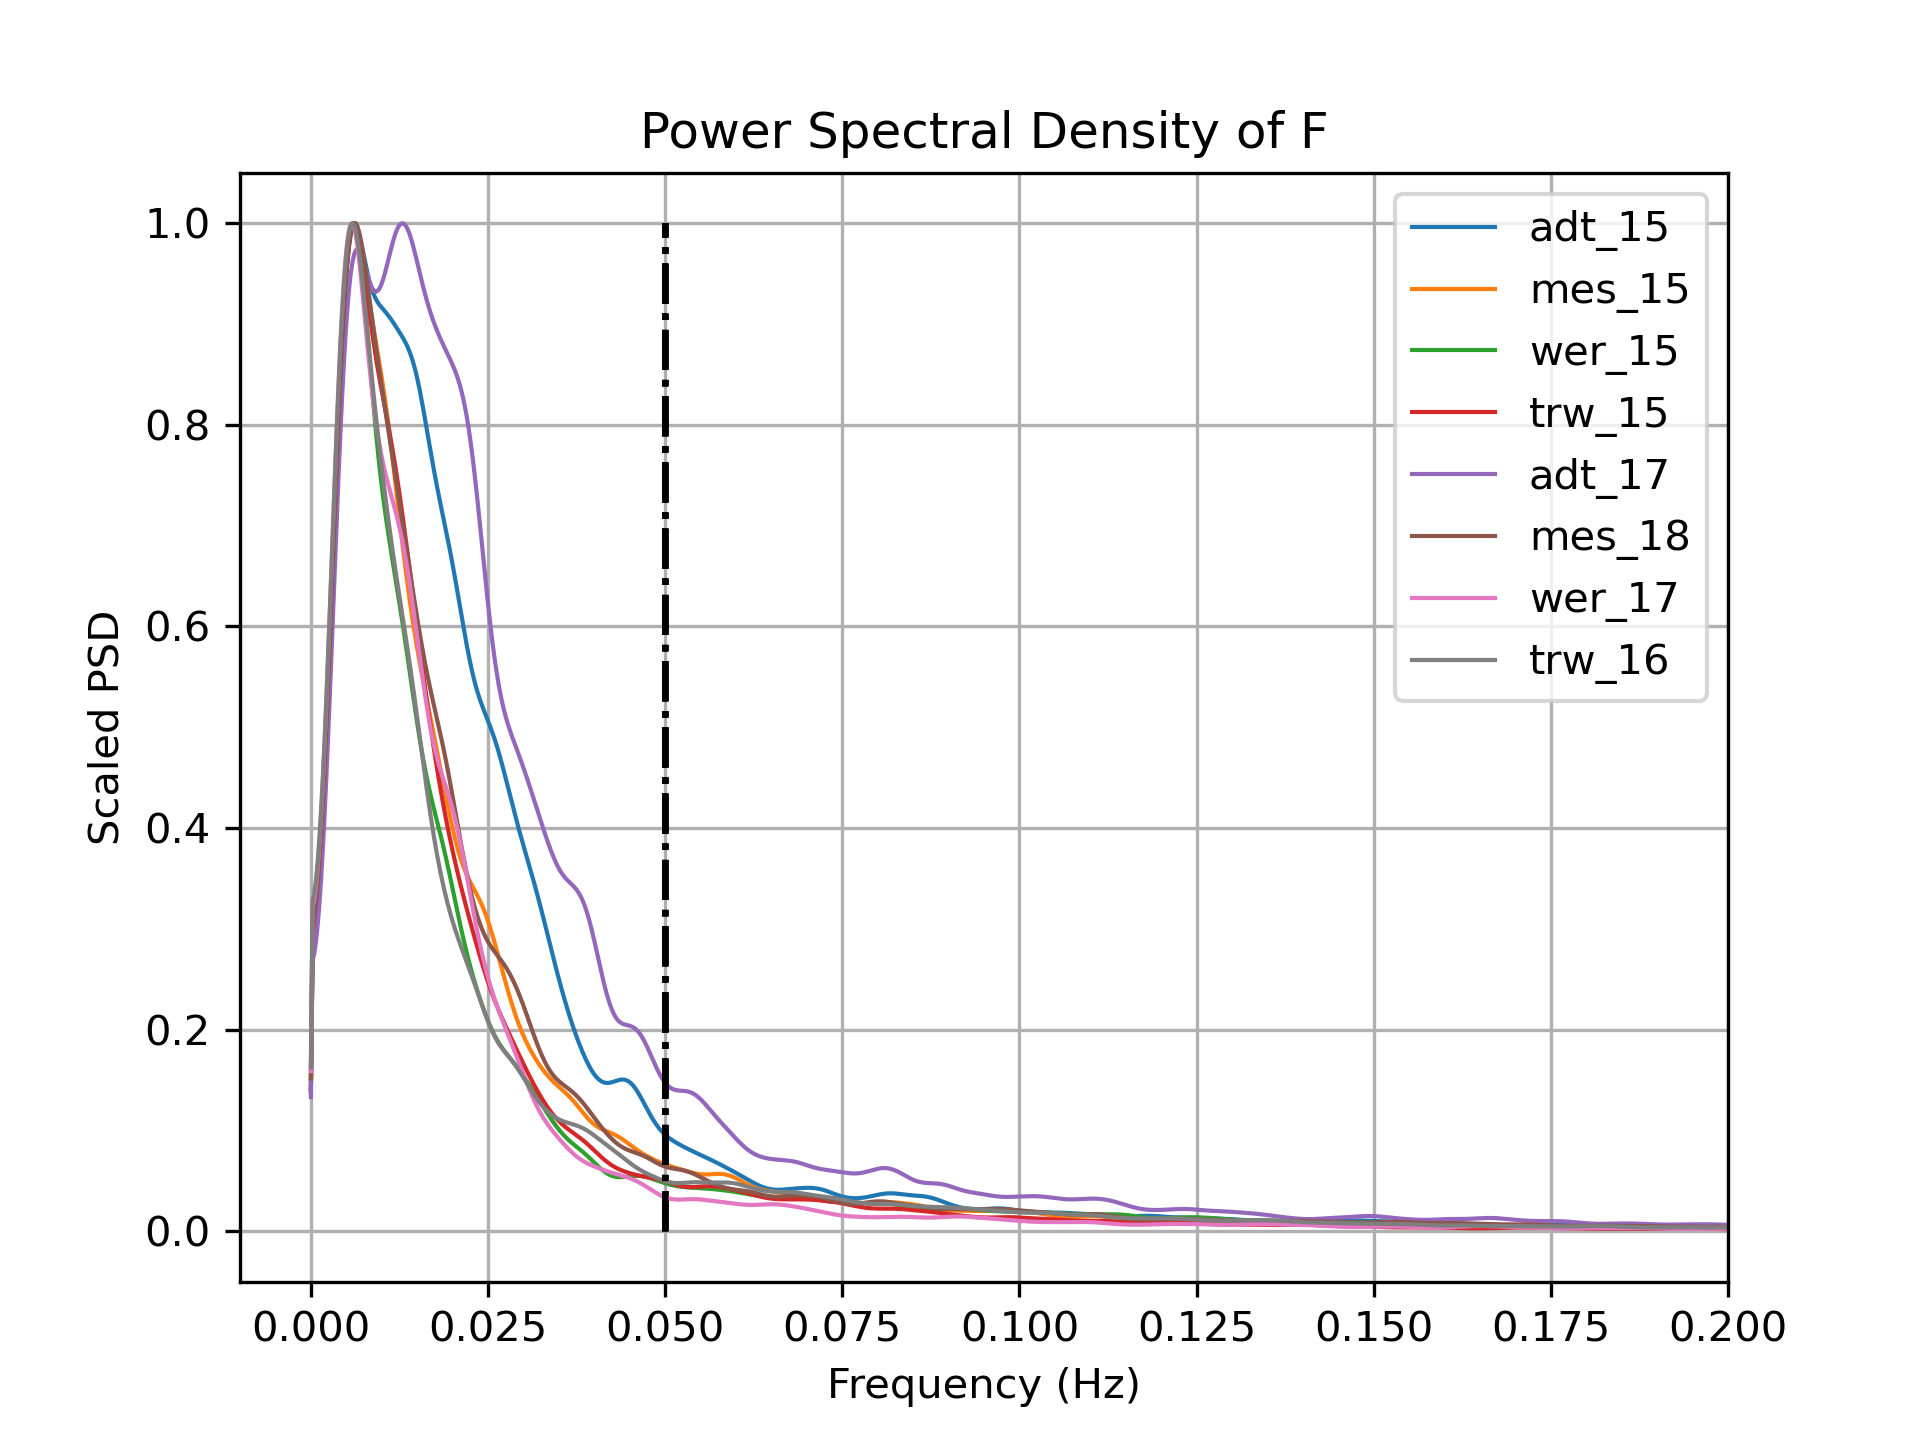
\includegraphics[width=0.48\textwidth]{./figs/bfr_smth/truck_psd/F.png}
        \caption{PSD of mass flow rate}
       \end{figure}
\end{multicols}

\begin{figure}[H]
        \centering
        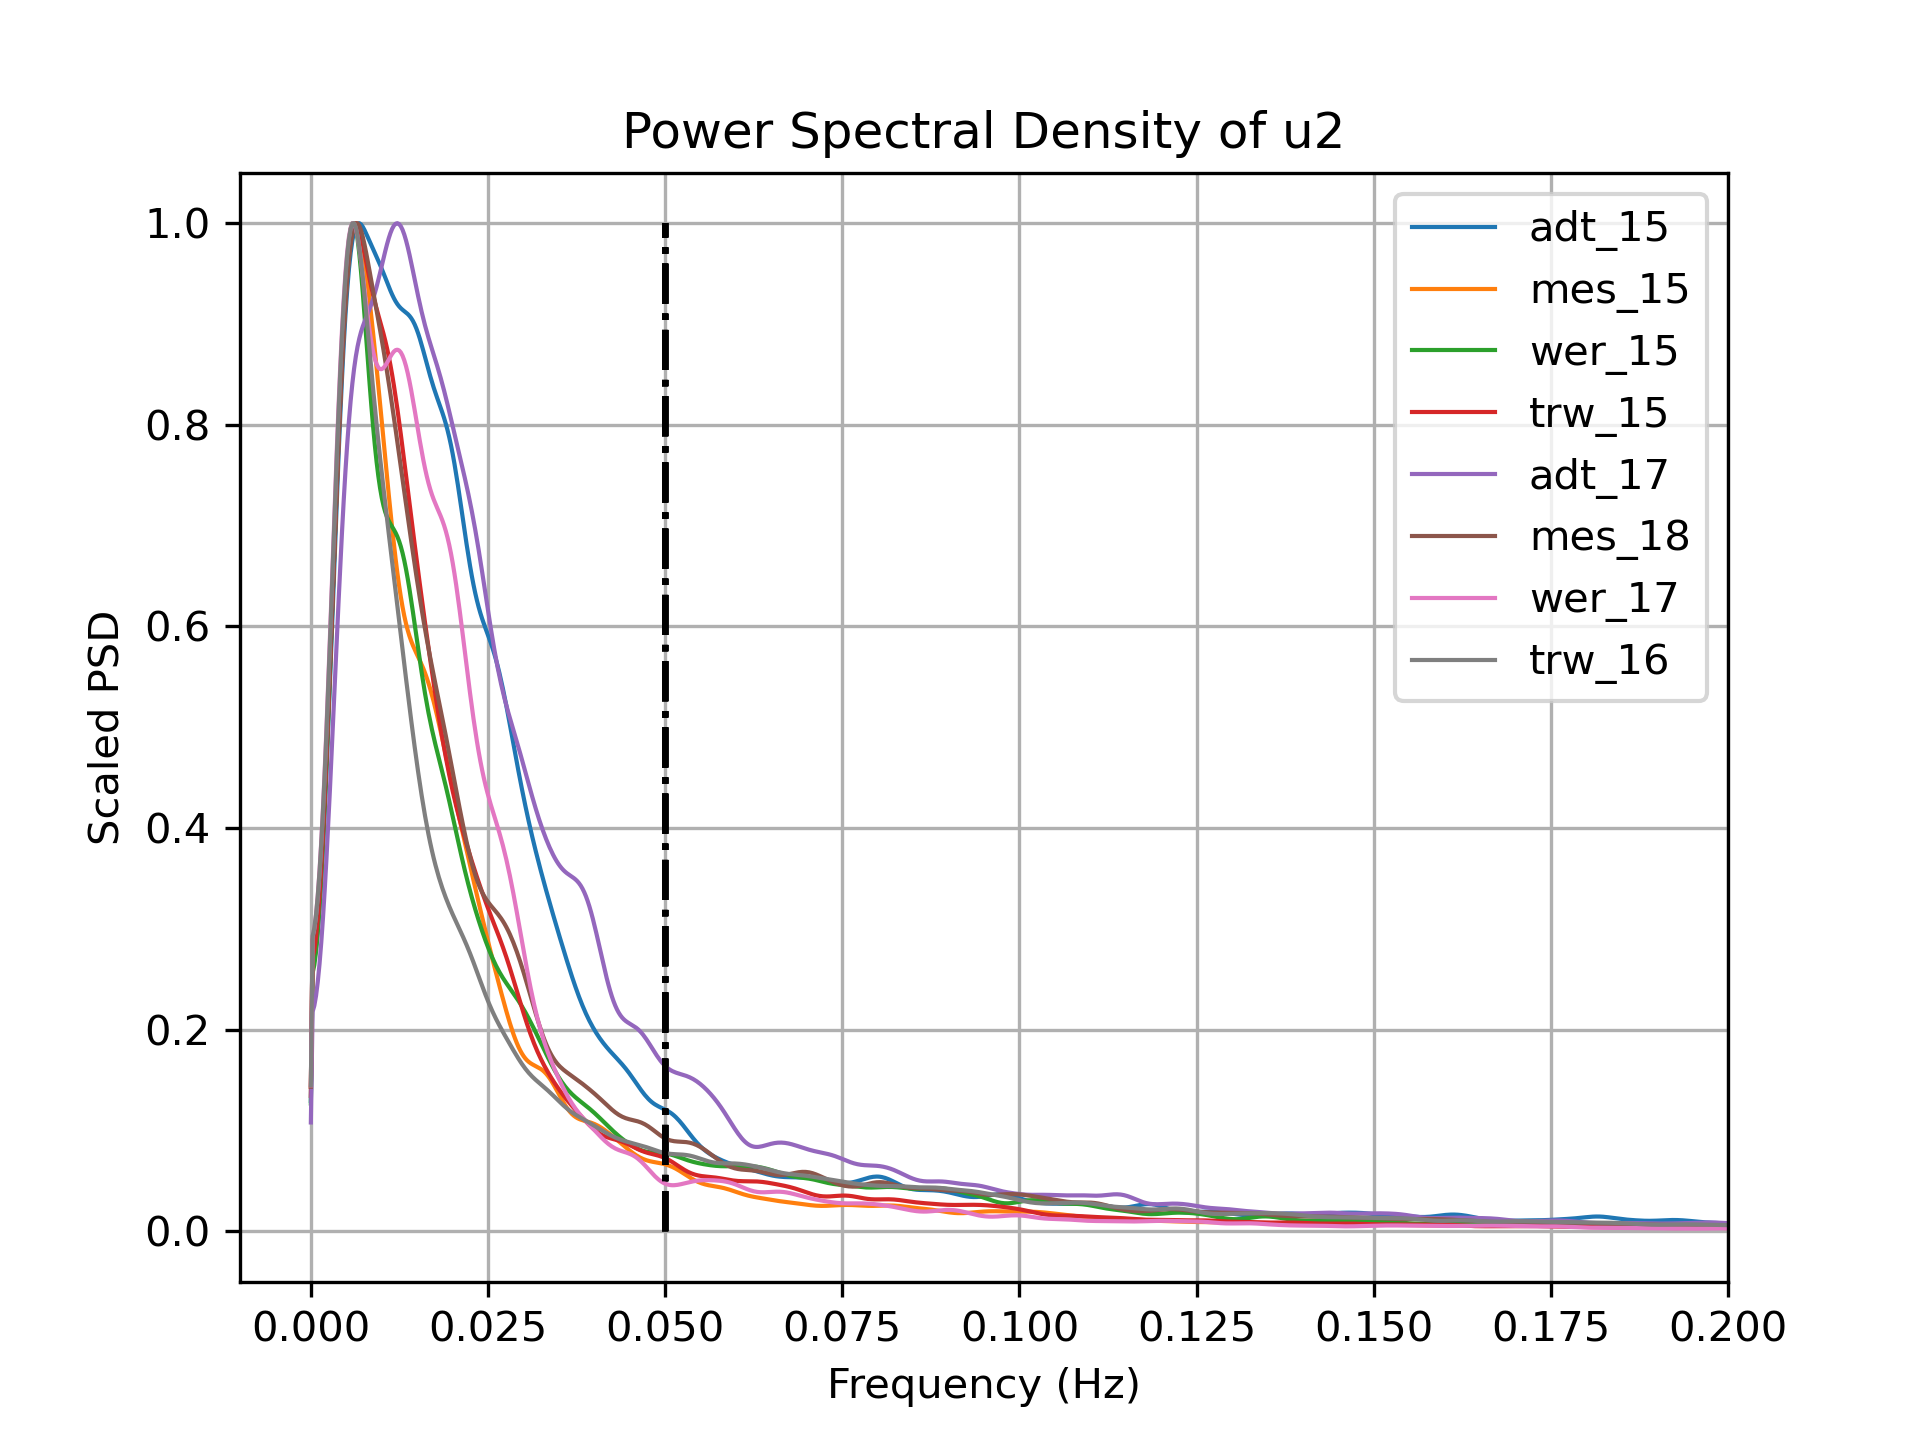
\includegraphics[width=0.6\textwidth]{./figs/bfr_smth/truck_psd/u2.png}
        \caption{PSD of $[NO_x]^{out}$}
\end{figure}


% ============================================================================

\subsubsection{Forgetting factor for RLS}

The PSD plots show that much of the energy for the signals in within the frequency range of $0 \, Hz$ to $0.05 \, Hz$. Thus, the forgetting factor for the RLS algorithm is chosen such that the equivalent time-constant is greater than $1/0.05 = 20 \, s$. We have,

\begin{align*}
        T_f &= \frac{t_d}{1 - \lambda}\\
        T_f = 20 \quad &\text{ and } \quad t_d = 1\\
        \implies \lambda &= 1 - \frac{t_d}{T_f} = 1 - \frac{1}{20} = 0.95
\end{align*}


% ============================================================================

\subsubsection{$h$ and $\nu$ parameters for individual signals}

\begin{table}[H]
        \centering
       \begin{tabular}{c c c}
              \hline \hline
              \itbf{signal}& $h$   & $\nu$   \\ \hline \hline
              $y_1$        & $5$   & $2.5$   \\
              $u_1$        & $40$  & $20$    \\
              $u_2$        & $2$   & $1$     \\
              $T$          & $40$  & $30$    \\
              $F$          & $400$ & $200$   \\ \hline \hline
       \end{tabular}
\caption{Values of threshold ($h$)  and bias ($\nu$) for individual truck data signals}
\end{table}
